\section{Prior Work}\label{sec:background_prior_work}
\textit{Assigned to: David}
\subsection{FCC fixed broadband deployment map}
 The \FCC maintains a map of broadband internet deployment across the United States \cite{FederalCommunicationsCommission}. This map is drawn at a census block level and only considers residential broadband.
 
 \subsection{Internet Connectivity MQP 2019}
In 2019, a similar MQP was run at WPI also with the goal of mapping the internet connectivity across the United States. They used traceroutes from Worcester to top websites and also did DNS cache manipulation to collect there data. They had mixed success collecting data, but they were ultimately able to produce the map below of all of there DNS data interpolated to cover the entire United States. They did not come to any conclusions as to the best or worst states. \cite{}

\begin{figure}[H]
    \centering
    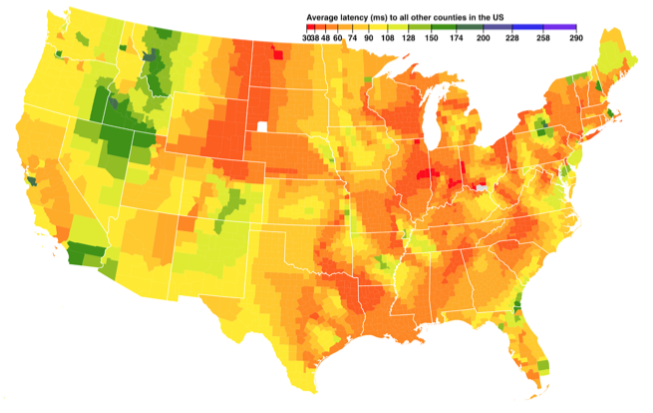
\includegraphics[width=\textwidth]{images/2019_MQP_DNS_Map.png}
    \caption{2019 MQP Interpolated DNS Map}
    \label{fig:2019_MQP_DNS_Map}
\end{figure}
 
\subsection{Physical Mapping of the Internets Fiber Backbone in the United States}
In 2015 researchers at the University of Wisconsin - Madison set out to map the locations of the fiber backbone within the United States  There goal was to understand how the physical locations of the fiber backbone had been influenced by previous infrastructure such as railroads and the highway network. They found strong correlation between the location of fiber lines and the locations of major roads built in the mid 20th century. This result is significant for internet connectivity because it further highlights that cities that were well connected physically during the industrial revolution  continue to be the best connected. 
 